\chapter{Process Control Engineering}
\label{Chapter:Controls}

There are two main goals in process control engineering:
\begin{enumerate*}
    \item Reference tracking, where a process variable is matched to a set-point which may be changed over time; and 
    \item Disturbance rejection, where the process variable is held to the set-point despite outside influence upsetting it;
\end{enumerate*}
This is usually achieved by a controller which detects the process variable using a sensor/transmitter and controls the process variable by manipulating an actuator. 

\section{Feedback}
\begin{figure}[h!]
    \centering
    
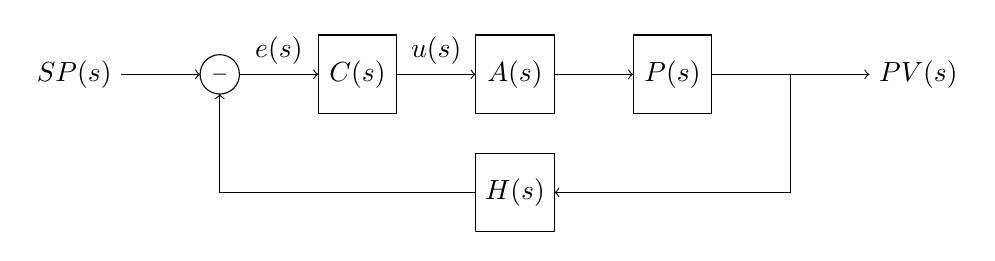
\begin{tikzpicture}
    
    %Sum
    \draw[->] (-3,0) node[anchor=east]{$SP(s)$}-- (-2,0);
    \draw (-1.75,0) circle (0.25)node{\scriptsize$-$};
    %Controller
    \draw[->] (-1.5,0) -- (-0.5,0)node[pos=0.5,anchor=south]{$e(s)$};
    \draw (-0.5,-0.5) rectangle (0.5,0.5) node[pos=0.5]{$C(s)$};
    \draw[->] (0.5,0) -- (1.5,0) node[pos=0.5,anchor=south]{$u(s)$};
    %Actuator
    \draw (1.5,-0.5) rectangle (2.5,0.5) node[pos=0.5]{$A(s)$};
    \draw[->] (2.5,0) -- (3.5,0);
    %Process
    \draw (3.5,-0.5) rectangle (4.5,0.5) node[pos=0.5]{$P(s)$};
    \draw[->] (4.5,0) -- (6.5,0) node[anchor=west]{$PV(s)$};
    %Transducer
    \draw[->] (5.5,0) -- (5.5,-1.5) -- (2.5,-1.5);
    \draw (1.5,-2) rectangle (2.5,-1) node[pos=0.5]{$H(s)$} ;
    \draw[->] (1.5,-1.5) -- (-1.75,-1.5) -- (-1.75,-0.25);
\end{tikzpicture}

    \caption[Feedback control loop]{Feedback control loop. The output ($PV$) is measured by the transducer ($H$) and compared to the set-point ($SP$). The controller ($C$) uses the actuator ($A$) to control the process ($P$) based on the error ($e$).}
    \label{fig:tikz_feedback}
\end{figure}

The most common type of controller is a feedback controller. Figure \ref{fig:tikz_feedback} shows a simple feedback control loop with a sensor/transmitter (\ie transducer), controller, and actuator working together to control a process. The controller takes action based on the `error' ($e$) between the set-point ($SP$) and process-variable ($PV$) (\ref{eqn:error}).

\begin{equation}\label{eqn:error}
    e(t) = PV(t) - SP(t)
\end{equation}

The action, or controller output ($u$) is often determined by a \acf{pid} equation (\ref{eqn:pid}), which considers the instantaneous, cumulative, and predictive error in determining the proper actuation \cite{Bequette}. This equation has three terms:
\begin{enumerate}
\item Proportional control term. The control output is manipulated in proportion to the error defined by the proportional gain constant ($K_P$). A high gain yields an aggressive controller that is prone to overshooting the set-point, while a low gain may result in steady-state offset.  
\item Integral control term, which considers the historical cumulative error (calculated by taking the time integral of the error) in an effort to eliminate steady-state offset that a P-Only controller may exhibit. As the process variable settles around the set-point, the cumulative error approaches a constant value and the effect of the integral controller diminishes.
\item Derivative control term, which estimates the time rate of change of the error to dampen overshoot. This mechanism, sometimes referred to as anticipatory control, slightly reduces the proportional response to the error when the error is changing rapidly. This results in reducing the peak overshoot. A wel tuned anticipatory gain can allow a more aggressive proportional gain to be used without the large overshoot.
\end{enumerate}

\begin{equation}\label{eqn:pid}
    u(t) 
    = \underbrace{K_P e(t)}_{\text{Proportional}} 
    + \underbrace{K_I \int_0^t e(t)dt}_{\text{Integral}} 
    + \underbrace{K_D \frac{de(t)}{dt}}_{\text{Derivative}}
\end{equation}

Instead of using three different gain constants, it is common for controllers to be tuned in terms of a single controller gain ($K_C$) plus two time constants: 
\begin{enumerate*}
    \item The integral time constant ($\tau_I$); and
    \item The derivative time constant ($\tau_D$);
\end{enumerate*}
In this case, \ref{eqn:pid} is rewritten as:
\begin{equation}\label{eqn:pid-tau}
    u(t) = K_C \left( e(t) + \tau_I^{-1} \int_0^t e(t)dt + \tau_D \frac{de(t)}{dt}\right)
\end{equation}

\section{Feedforward}
The term `Feedforward' can be used to refer to any element in the control block diagram that exists outside of the feedback loop. In process control, feedforward controllers are almost always implemented alongside, not instead of feedback controllers because a standalone feedforward controller is not guaranteed to reach the set-point.  

\subsection{Disturbance Feedforward}
\begin{figure}[h!]
    \centering
    
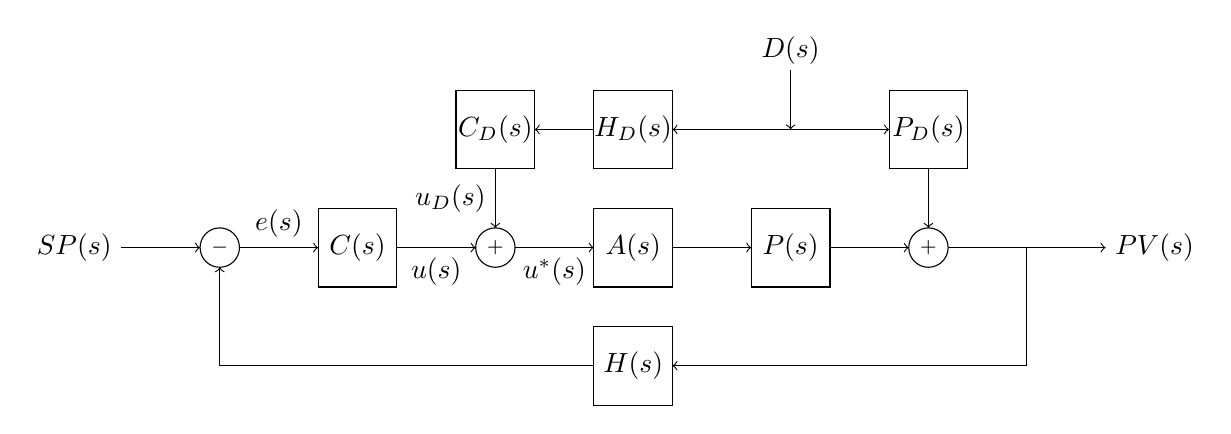
\begin{tikzpicture}
    
    %Error Sum
    \draw[->] (-4.5,0) node[anchor=east]{$SP(s)$}-- (-3.5,0);
    \draw (-3.25,0) circle (0.25) node{\scriptsize$-$};
    %Controller
    \draw[->] (-3,0) -- (-2,0)node[pos=0.5,anchor=south]{$e(s)$};
    \draw (-2,-0.5) rectangle (-1,0.5) node[pos=0.5]{$C(s)$};
    \draw[->] (-1,0) -- (0,0) node[pos=0.5,anchor=north]{$u(s)$};
    %Control Sum
    \draw (0.25,0) circle (0.25) node{\scriptsize$+$}; 
    %Actuator
    \draw[->] (0.5,0) -- (1.5,0)node[pos=0.5,anchor=north]{$u^*(s)$};
    \draw (1.5,-0.5) rectangle (2.5,0.5) node[pos=0.5]{$A(s)$};
    \draw[->] (2.5,0) -- (3.5,0);
    %Process
    \draw (3.5,-0.5) rectangle (4.5,0.5) node[pos=0.5]{$P(s)$};
    \draw[->] (4.5,0) -- (5.5,0);
    \draw[->] (6,0) -- (8,0)node[anchor=west]{$PV(s)$};
    %Output Sum
    \draw (5.75,0) circle (0.25) node{\scriptsize$+$};
    %Transducer
    \draw[->] (7,0) -- (7,-1.5) -- (2.5,-1.5);
    \draw (1.5,-2) rectangle (2.5,-1) node[pos=0.5]{$H(s)$} ;
    \draw[->] (1.5,-1.5) -- (-3.25,-1.5) -- (-3.25,-0.25);
    %Disturbance Transducer
    \draw (1.5,1) rectangle (2.5,2) node[pos=0.5]{$H_D(s)$} ;
    \draw[->] (1.5,1.5) -- (0.75,1.5);
    %Disturbance Controller
    \draw (-0.25,1) rectangle (0.75,2) node[pos=0.5]{$C_D(s)$};
    \draw[->] (0.25,1) -- (0.25,0.25)node[pos=0.5,anchor=east]{$u_D(s)$};
    %Disturbance Dynamics
    \draw (5.25,1) rectangle (6.25,2) node[pos=0.5]{$P_D(s)$};
    \draw[->] (5.75,1) -- (5.75,0.25);
    %Disturbance
    \node at (4,2.5) {$D(s)$};
    \draw[<->] (2.5,1.5) -- (5.25,1.5);
    \draw[->] (4,2.25) -- (4,1.5);
\end{tikzpicture}

    \caption[Feedback control loop with disturbance feedforward]{Feedback control loop with disturbance feedforward. It is identical to Fig. \ref{fig:tikz_feedback} with the addition of a disturbance ($D$) which effects the process variable ($PV$) according to the disturbance dynamics ($P_D$), and is measured by the disturbance transducer ($H_D$). The signal from $H_D$ is sent to the disturbance feedforward controller ($C_D$) who's output ($u_D$) is combined with ($u$) to form the total control output ($u^*$).}
    \label{fig:tikz_feedforward}
\end{figure}

In many processes, the process variable is effected by phenomena other than the actuator. These other phenomena are defined as disturbances. A well-tuned feedback controller is capable of disturbance rejection, but only after the disturbance causes error. In some cases, a disturbance feedforward controller may be added to the feedback controller to cause the actuator to counteract the effect of the disturbance before it occurs \cite{Bequette}.

The most prevalent disturbances that would effect the power output of the core of a \acs{msnb} are the temperature reactivity feedback effect common to all nuclear reactors and the flow reactivity specific to natural circulation driven  liquid fueled \acsp{msr} \cite{CarterNumerical}. Temperature reactivity feedback is dominated by Doppler Broadening, where the microscopic radiative capture cross section resonance peaks of nuclides such as \U[238] are depressed to cover a wider epithermal neutron spectrum \cite{DH}. This results in a smaller core neutron population and less fission events, so there is a negative correlation between fuel temperature and fuel reactivity. Flow reactivity is driven by the advection of delayed neutron precursors. Not all fission neutrons are released promptly; sometimes an unstable nuclide which decays by neutron emission produced instead. These unstable nuclides are called delayed neutron precursors and have half-lives ranging from less than a second to over a minute \cite{Lamarsh}. Since the fuel in a \acs{msnb} is flowing, there is a statistical probability that a delayed neutron precursor may leave the core by advection before the neutron is emitted in a much less reactive part of the reactor. When the temperature differential between the thermal center of the core and primary heat exchanger is increased, so too does the natural circulation flow rate. This decreases the likelihood of delayed neutrons being emitted in the core, and negatively contributes to core reactivity. Devices meant to elongate the in-core flow path may minimize delayed neutron losses \cite{CarterPHD}.

Disturbance feedforward will not be utilized in the design of the controller outlined in this work. When the outlet temperature of the heat exchanger is decreased, it takes time for the cooler salt to reach the core. The disturbance transport delay is on the order of minutes. Contrastly, Doppler Broadening has a nearly instantaneous effect, so disturbance dynamics are on the order of milliseconds, governed by the mean neutron lifetime \cite{DH,Lamarsh}. The effect of control actuation are similarly prompt. Even with a temperature sensor just at the inlet of the core it would be nearly impossible to reliably predict the exact moment that control reactivity would be need to be inserted to counteract the temperature reactivity. 

\subsection{Pre-Filter}
\begin{figure}[h!]
    \centering
    \input{tikz/prefilter}
    \caption[Feedback control loop with pre-filter]{Feedback control loop with pre-filter. It is identical to Fig. \ref{fig:tikz_feedback} with the addition of the pre-filter ($F$) which reshapes changes to the set-point ($SP$) before calculating the error ($e$).}
    \label{fig:tikz_prefilter}
\end{figure}

Pre-filters are another type of feedforward mechanism common in control systems. They are typically first-order transfer functions such as \ref{eqn:prefilter} function used to improve the performance of the associated feedback controller (as depicted by Figure \ref{fig:tikz_prefilter} by `slowing down' the rate of change of the set-point. The gain (numerator) for a pre-filter is always unity because the desire is only to reshape the input, not resize it. The time-constant ($\tau_F$) describes how quickly the output equilibrates with the input. 

\begin{equation}\label{eqn:prefilter}
    F(s)=\frac{1}{\tau_F s+1}    
\end{equation}

By braking instantaneous set-point changes, or step functions, the pre-filter minimizes the instantaneous error during transients and minimizes overshoot by reducing over-actuation or actuator saturation.  This is particularly useful in a control system such as the one designed in this report where the set-point is coupled to some other value. In this case, the core power generation needs to match the demand of the secondary system (\eg power cycle). This method allows the secondary system to immediately change to its necessary value while giving the reactor core time to safely and effectively respond. 

\begin{figure}[h!]
    \centering
    \subfloat[\centering Step-function]{{\resizebox{0.47\textwidth}{!}{% This file was created by matlab2tikz.
%
%The latest updates can be retrieved from
%  http://www.mathworks.com/matlabcentral/fileexchange/22022-matlab2tikz-matlab2tikz
%where you can also make suggestions and rate matlab2tikz.
%
\definecolor{mycolor1}{rgb}{0.00000,0.44700,0.74100}%
\definecolor{mycolor2}{rgb}{0.85000,0.32500,0.09800}%
%
\begin{tikzpicture}

\begin{axis}[%
width=4.521in,
height=3.566in,
at={(0.758in,0.481in)},
scale only axis,
xmin=0,
xmax=10,
xtick={ 0,  1,  2,  3,  4,  5,  6,  7,  8,  9, 10},
xticklabel style={font=\sansmath\sffamily},
xlabel style={font=\sansmath\sffamily},
xlabel={Time Constants, $\tau_F$},
ymin=-0.05,
ymax=1.05,
ylabel style={font=\sansmath\sffamily},
ylabel={Normalized Magnitude},
yticklabel style={font=\sansmath\sffamily},
ytick={0,0.632,0.865,0.95,1},
axis background/.style={fill=white},
legend style={at={(0.711,0.171)}, anchor=south west, legend cell align=left, align=left, font=\sansmath\sffamily}
]

\addplot [color=mycolor1]
  table[row sep=crcr]{%
0	0\\
0.2	0\\
0.4	0\\
0.6	0\\
0.8	0\\
0.999999999999993	0\\
1	1\\
1.00000000000001	1\\
1.20000000000001	1\\
1.40000000000001	1\\
1.60000000000001	1\\
1.80000000000001	1\\
2.00000000000001	1\\
2.20000000000001	1\\
2.40000000000001	1\\
2.60000000000001	1\\
2.80000000000001	1\\
3.00000000000002	1\\
3.20000000000002	1\\
3.40000000000002	1\\
3.60000000000002	1\\
3.80000000000002	1\\
4.00000000000002	1\\
4.20000000000002	1\\
4.40000000000002	1\\
4.60000000000002	1\\
4.80000000000002	1\\
4.99999999999996	1\\
5.00000000000002	1\\
5.20000000000002	1\\
5.40000000000002	1\\
5.60000000000002	1\\
5.80000000000002	1\\
6.00000000000002	1\\
6.20000000000002	1\\
6.40000000000002	1\\
6.60000000000002	1\\
6.80000000000002	1\\
7.00000000000002	1\\
7.20000000000002	1\\
7.40000000000002	1\\
7.60000000000002	1\\
7.80000000000002	1\\
8.00000000000002	1\\
8.20000000000002	1\\
8.40000000000002	1\\
8.60000000000002	1\\
8.80000000000002	1\\
9.00000000000002	1\\
9.20000000000002	1\\
9.40000000000001	1\\
9.60000000000001	1\\
9.80000000000001	1\\
10	1\\
};
\addlegendentry{Input}

\addplot [color=mycolor2, dashed]
  table[row sep=crcr]{%
0	0\\
0.2	0\\
0.4	0\\
0.6	0\\
0.8	0\\
0.999999999999993	0\\
1	0\\
1.00000000000001	1.42108547152019e-14\\
1.20000000000001	0.181269226666678\\
1.40000000000001	0.329679920797011\\
1.60000000000001	0.451188323173276\\
1.80000000000001	0.550670991417293\\
2.00000000000001	0.63212051332198\\
2.20000000000001	0.698805743378635\\
2.40000000000001	0.753402993352831\\
2.60000000000001	0.798103442046079\\
2.80000000000001	0.834701074973048\\
3.00000000000002	0.864664683281515\\
3.20000000000002	0.889196811483763\\
3.40000000000002	0.909282019778302\\
3.60000000000002	0.925726397897851\\
3.80000000000002	0.939189916312655\\
4.00000000000002	0.950212913156196\\
4.20000000000002	0.959237779886358\\
4.40000000000002	0.966626716003575\\
4.60000000000002	0.972676265384934\\
4.80000000000002	0.977629217628252\\
4.99999999999996	0.981684352048706\\
5.00000000000002	0.981684352048707\\
5.20000000000002	0.985004415388737\\
5.40000000000002	0.987722653414635\\
5.60000000000002	0.989948158535683\\
5.80000000000002	0.991770248064495\\
6.00000000000002	0.993262048833503\\
6.20000000000002	0.994483432030772\\
6.40000000000002	0.995483416040408\\
6.60000000000002	0.996302133721938\\
6.80000000000002	0.996972443082479\\
7.00000000000002	0.997521245983607\\
7.20000000000002	0.997970567807256\\
7.40000000000002	0.998338441411407\\
7.60000000000002	0.998639630851823\\
7.80000000000002	0.998886223915294\\
8.00000000000002	0.999088117244848\\
8.20000000000002	0.999253413526685\\
8.40000000000002	0.999388746679343\\
8.60000000000002	0.999499548096076\\
8.80000000000002	0.999590264625684\\
9.00000000000002	0.999664537040124\\
9.20000000000002	0.999725346151436\\
9.40000000000001	0.999775132442167\\
9.60000000000001	0.999815894010477\\
9.80000000000001	0.999849266760823\\
10	0.999876590058521\\
};
\addlegendentry{Output}

\end{axis}

\begin{axis}[%
width=5.833in,
height=4.375in,
at={(0in,0in)},
scale only axis,
xmin=0,
xmax=1,
ymin=0,
ymax=1,
axis line style={draw=none},
ticks=none,
axis x line*=bottom,
axis y line*=left
]
\end{axis}
\end{tikzpicture}%}}}
    \qquad
    \subfloat[\centering Ramp-function]{\resizebox{0.47\textwidth}{!}{% This file was created by matlab2tikz.
%
%The latest updates can be retrieved from
%  http://www.mathworks.com/matlabcentral/fileexchange/22022-matlab2tikz-matlab2tikz
%where you can also make suggestions and rate matlab2tikz.
%
\definecolor{mycolor1}{rgb}{0.00000,0.44700,0.74100}%
\definecolor{mycolor2}{rgb}{0.85000,0.32500,0.09800}%
%
\begin{tikzpicture}

\begin{axis}[%
width=4.521in,
height=3.566in,
at={(0.758in,0.481in)},
scale only axis,
xmin=0,
xmax=10,
xtick={ 0,  1,  2,  3,  4,  5,  6,  7,  8,  9, 10},
xlabel style={font=\color{white!15!black}},
xlabel={Time},
ymin=-0.1,
ymax=1.1,
ylabel style={font=\color{white!15!black}},
ylabel={Value},
axis background/.style={fill=white},
legend style={at={(0.711,0.171)}, anchor=south west, legend cell align=left, align=left, draw=white!15!black}
]
\addplot [color=mycolor1]
  table[row sep=crcr]{%
0	0\\
0.2	0\\
0.4	0\\
0.6	0\\
0.8	0\\
0.999999999999993	0\\
1	0\\
1.00000000000001	3.5527136788005e-15\\
1.20000000000001	0.0500000000000035\\
1.40000000000001	0.100000000000004\\
1.60000000000001	0.150000000000004\\
1.80000000000001	0.200000000000004\\
2.00000000000001	0.250000000000004\\
2.20000000000001	0.300000000000004\\
2.40000000000001	0.350000000000004\\
2.60000000000001	0.400000000000004\\
2.80000000000001	0.450000000000004\\
3.00000000000002	0.500000000000004\\
3.20000000000002	0.550000000000004\\
3.40000000000002	0.600000000000004\\
3.60000000000002	0.650000000000004\\
3.80000000000002	0.700000000000004\\
4.00000000000002	0.750000000000004\\
4.20000000000002	0.800000000000004\\
4.40000000000002	0.850000000000004\\
4.60000000000002	0.900000000000004\\
4.80000000000002	0.950000000000004\\
4.99999999999996	0.99999999999999\\
5.00000000000002	1\\
5.20000000000002	1\\
5.40000000000002	1\\
5.60000000000002	1\\
5.80000000000002	1\\
6.00000000000002	1\\
6.20000000000002	1\\
6.40000000000002	1\\
6.60000000000002	1\\
6.80000000000002	1\\
7.00000000000002	1\\
7.20000000000002	1\\
7.40000000000002	1\\
7.60000000000002	1\\
7.80000000000002	1\\
8.00000000000002	1\\
8.20000000000002	1\\
8.40000000000002	1\\
8.60000000000002	1\\
8.80000000000002	1\\
9.00000000000002	1\\
9.20000000000002	1\\
9.40000000000001	1\\
9.60000000000001	1\\
9.80000000000001	1\\
10	1\\
};
\addlegendentry{Input}

\addplot [color=mycolor2, dashed]
  table[row sep=crcr]{%
0	0\\
0.2	0\\
0.4	0\\
0.6	0\\
0.8	0\\
0.999999999999993	0\\
1	0\\
1.00000000000001	2.52378540224252e-29\\
1.20000000000001	0.00468269333333398\\
1.40000000000001	0.0175800198007507\\
1.60000000000001	0.0372029192066846\\
1.80000000000001	0.0623322521456803\\
2.00000000000001	0.0919698716695085\\
2.20000000000001	0.125298564155345\\
2.40000000000001	0.161649251661796\\
2.60000000000001	0.200474139488484\\
2.80000000000001	0.241324731256742\\
3.00000000000002	0.283833829179625\\
3.20000000000002	0.327700797129063\\
3.40000000000002	0.372679495055428\\
3.60000000000002	0.418568400525541\\
3.80000000000002	0.46520252092184\\
4.00000000000002	0.512446771710955\\
4.20000000000002	0.560190555028414\\
4.40000000000002	0.60834332099911\\
4.60000000000002	0.656830933653771\\
4.80000000000002	0.705592695592941\\
4.99999999999996	0.754578911987813\\
5.00000000000002	0.754578911987827\\
5.20000000000002	0.799066202819486\\
5.40000000000002	0.835489316845594\\
5.60000000000002	0.865310041159399\\
5.80000000000002	0.8897251858382\\
6.00000000000002	0.90971461612212\\
6.20000000000002	0.926080577836966\\
6.40000000000002	0.939479894328106\\
6.60000000000002	0.950450327081035\\
6.80000000000002	0.959432157972642\\
7.00000000000002	0.966785859324477\\
7.20000000000002	0.972806560919127\\
7.40000000000002	0.977735894591724\\
7.60000000000002	0.981771691761507\\
7.80000000000002	0.98507592309934\\
8.00000000000002	0.987781198977837\\
8.20000000000002	0.989996091589918\\
8.40000000000002	0.991809492331058\\
8.60000000000002	0.993294179322215\\
8.80000000000002	0.994509738250642\\
9.00000000000002	0.995504953752146\\
9.20000000000002	0.996319767309325\\
9.40000000000001	0.996986880243117\\
9.60000000000001	0.997533066131301\\
9.80000000000001	0.997980245325918\\
10	0.998346364693745\\
};
\addlegendentry{Output}

\end{axis}

\begin{axis}[%
width=5.833in,
height=4.375in,
at={(0in,0in)},
scale only axis,
xmin=0,
xmax=1,
ymin=0,
ymax=1,
axis line style={draw=none},
ticks=none,
axis x line*=bottom,
axis y line*=left
]
\end{axis}
\end{tikzpicture}%}}
    \caption[Pre-filter on step-function and ramp-function]{Pre-filter on step-function and ramp-function.}
    \label{fig:pgf_prefilter}
\end{figure}

\section{Time Variance}
Fissile depletion - time function parameters or look-up table to gain-schedule and turn the time variant system into a shift invariant system.

In addition to the relatively slow time variance of fissile fuel depletion during steady-state critical operation, there are specific times in a \acs{msnb}'s expected operational life-cycle that exhibit a higher degree of time variance: 
\begin{enumerate*}
\item Start-up; \item Shut-down; and \item Re-start.
\end{enumerate*}

\subsection{Start-up}
Black-start may need to deal with thawing salt - main concern is fission product neutron poison build-up (discuss the burnable poison stuff)

\subsection{Shut-down}
Planned shut-down

Emergency Shutdown/SCRAM(must be passive)

Decay heat and keeping the salt liquid for restart

\subsection{Re-start}
\Xe stripper


